\chapter{Results}

All of the obtained sequences were analyzed using Multiple Sequence Alignment. 
There were 2 different approaches used for the analysis. 
One involved using ClustalOmega analysis with no bootstrapping.
A second analysis was performed in program MEGA11 using the MUSCLE approach with bootstrapping.  
Both approaches produced phylogenetic trees which were colored in the program FigTree and compared.

\section{Phylogenetic tree created using ClustalOmega - no bootstrapping.}

Following the sequence alignment using the ClustalOmega method a phylogenetic tree was produced and exported to the Figtree program. 
It is important to note that this data was not analyzed using the bootstrap method in the program MEGA11 and was directly exported from the online website which performed the analysis. \\
Each of the branches was colored using this program accordingly with the color code allocated for the country the branch was representing. 
Figure 4.1 shows two different ways of displaying phylogenetic trees. 
Part A of Figure 4.1 represents a polar tree layout whereas Part B represents a rectangular tree layout. 
Part C represents a color-coded legend for each country within the phylogenetic tree. 
Rectangular tree layout does not contain tree branch labels as they were to compressed to be read.\\
As seen in Figure 4.1 some of the countries or regions of the countries have formed clades. 
One such clade seen on the left side of the polar layout tree which can be clearly distinguished was color-coded using dark blue color. 
This region contained sequences from Serbia. 
A part of this clade contained a few sequences from Slovenia which were color-coded in orange. 
On the opposite side of the tree another, small Balkan clade could be distinguished, which contained sequences mainly from Croatia and one sequence from Slovenia. 
Another interesting clade was located below the Serbian-Slovenian branch, which included many sequences from Estonia (color-coded in pink) alongside with few sequences from Russia,  Belarus, and Ukraine. 
There were many smaller clades that were specific to one country such as Polish branches and a few Romanian ones. \\
For the most part, the branches of the tree were expected to point outwards, however, below the Croatian-Slovenian clade, there was a Hungarian-Slovakian clade that contained an example of back-mutations. 
Another example of back-mutations could be seen on the top left side of the polar tree within the Ukrainian-Hungarian clade (color-coded in blue and purple). 
Both of the Hungarian sequences seemed to mutate back.

\begin{figure}[h]
  \centering
  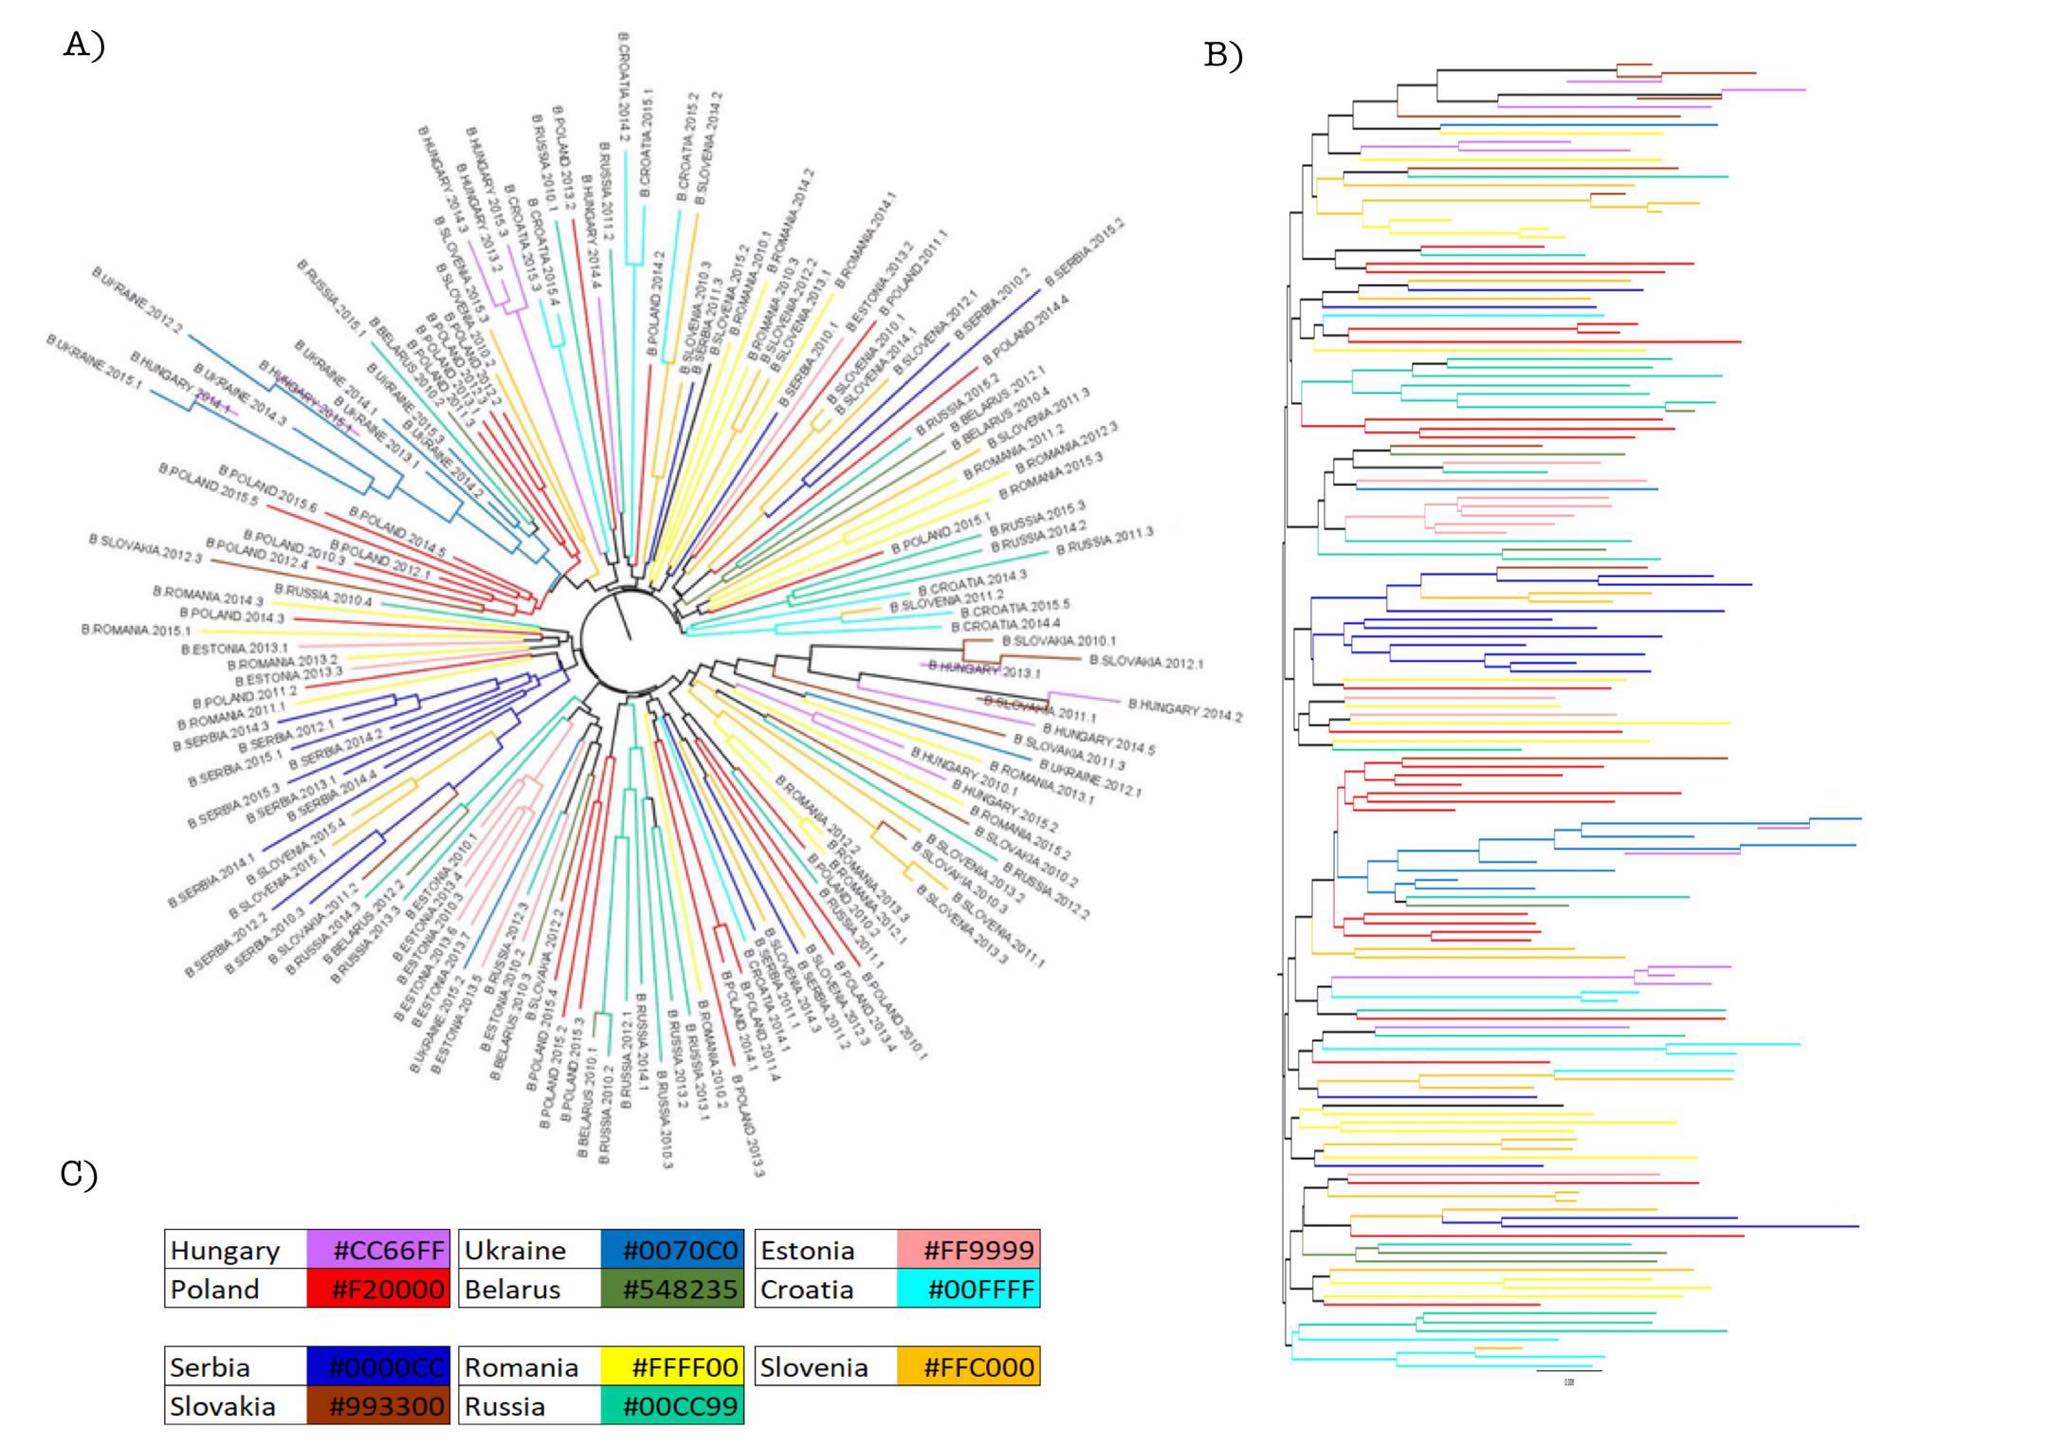
\includegraphics[width=0.8\textwidth]{images/before bootstrapping all.jpeg}
  \caption{Phylogenetic tree (before bootstrapping) aligned using ClustalOmega and colored in the FigTree program. A) Polar tree layout which includes the names of the countries at the tip of the branches. B) Rectangular tree layout which does not include the name of the countries at the tip of the branches. C) Legend describing which color was used for which country.}
  \label{fig: No bootstrapping trees.}
\end{figure}
 
\section{Phylogenetic tree created using MUSCLE - with bootstrapping.}

Another tree was constructed with the use of the program MEGA11. 
As mentioned in the “Methods” section, Multiple Sequence Analysis was performed using the program MEGA11 using the MUSCLE method, followed by Maximum Likelihood Test and Bootstrap analysis. \\
Figure 4.2 also shows both the polar and rectangular layout of the tree which was produced alongside the color-code legend. 
Due to bootstrapping, the construction of the tree shown in Figure 4.2 was slightly different from the tree shown in Figure 4.1. 
The sequences which were previously referred to as Serbian clades were redistributed to other parts of the tree. 
As a result, the formation of the Serbian-Croatian-Slovenian clade could be observed. 
The Estonian clade did not change as much. \\
Another interesting clade that was not mentioned previously, but remained relatively the same was the Polish-Russian clade, which was located towards the top of the polar tree. 
This clade contains also one Belarusian sequence. 
\\
What is very different from the previous figure, Figure 4.2 does not contain any reverse mutations within the tree. 
A Hungarian sequence B.HUNGARY.2013.1 was previously positioned within one clade with the Slovakian sequences. 
After bootstrapping, this sequence moved into one clade with a Ukrainian clade.
Another Hungarian sequence which showed back-mutation in Figure 4.1, B.HUNGARY.2015.1 as well as sequence B.HUNGARY.2014.1, which were previously within the Ukrainian clade, moved within different clades after bootstrapping.
All three of the sequences showed back-mutations before bootstrapping, but not after. 
A Slovakian sequence B.SLOVAKIA.2011.1 presented as back-mutation before bootstrapping (see. Figure 4.1), but not after. 
Previously, this sequence was within the Slovakian-Hungarian clade, but after bootstrapping, it moved to the Ukrainian clade.


\begin{figure}[h]
  \centering
  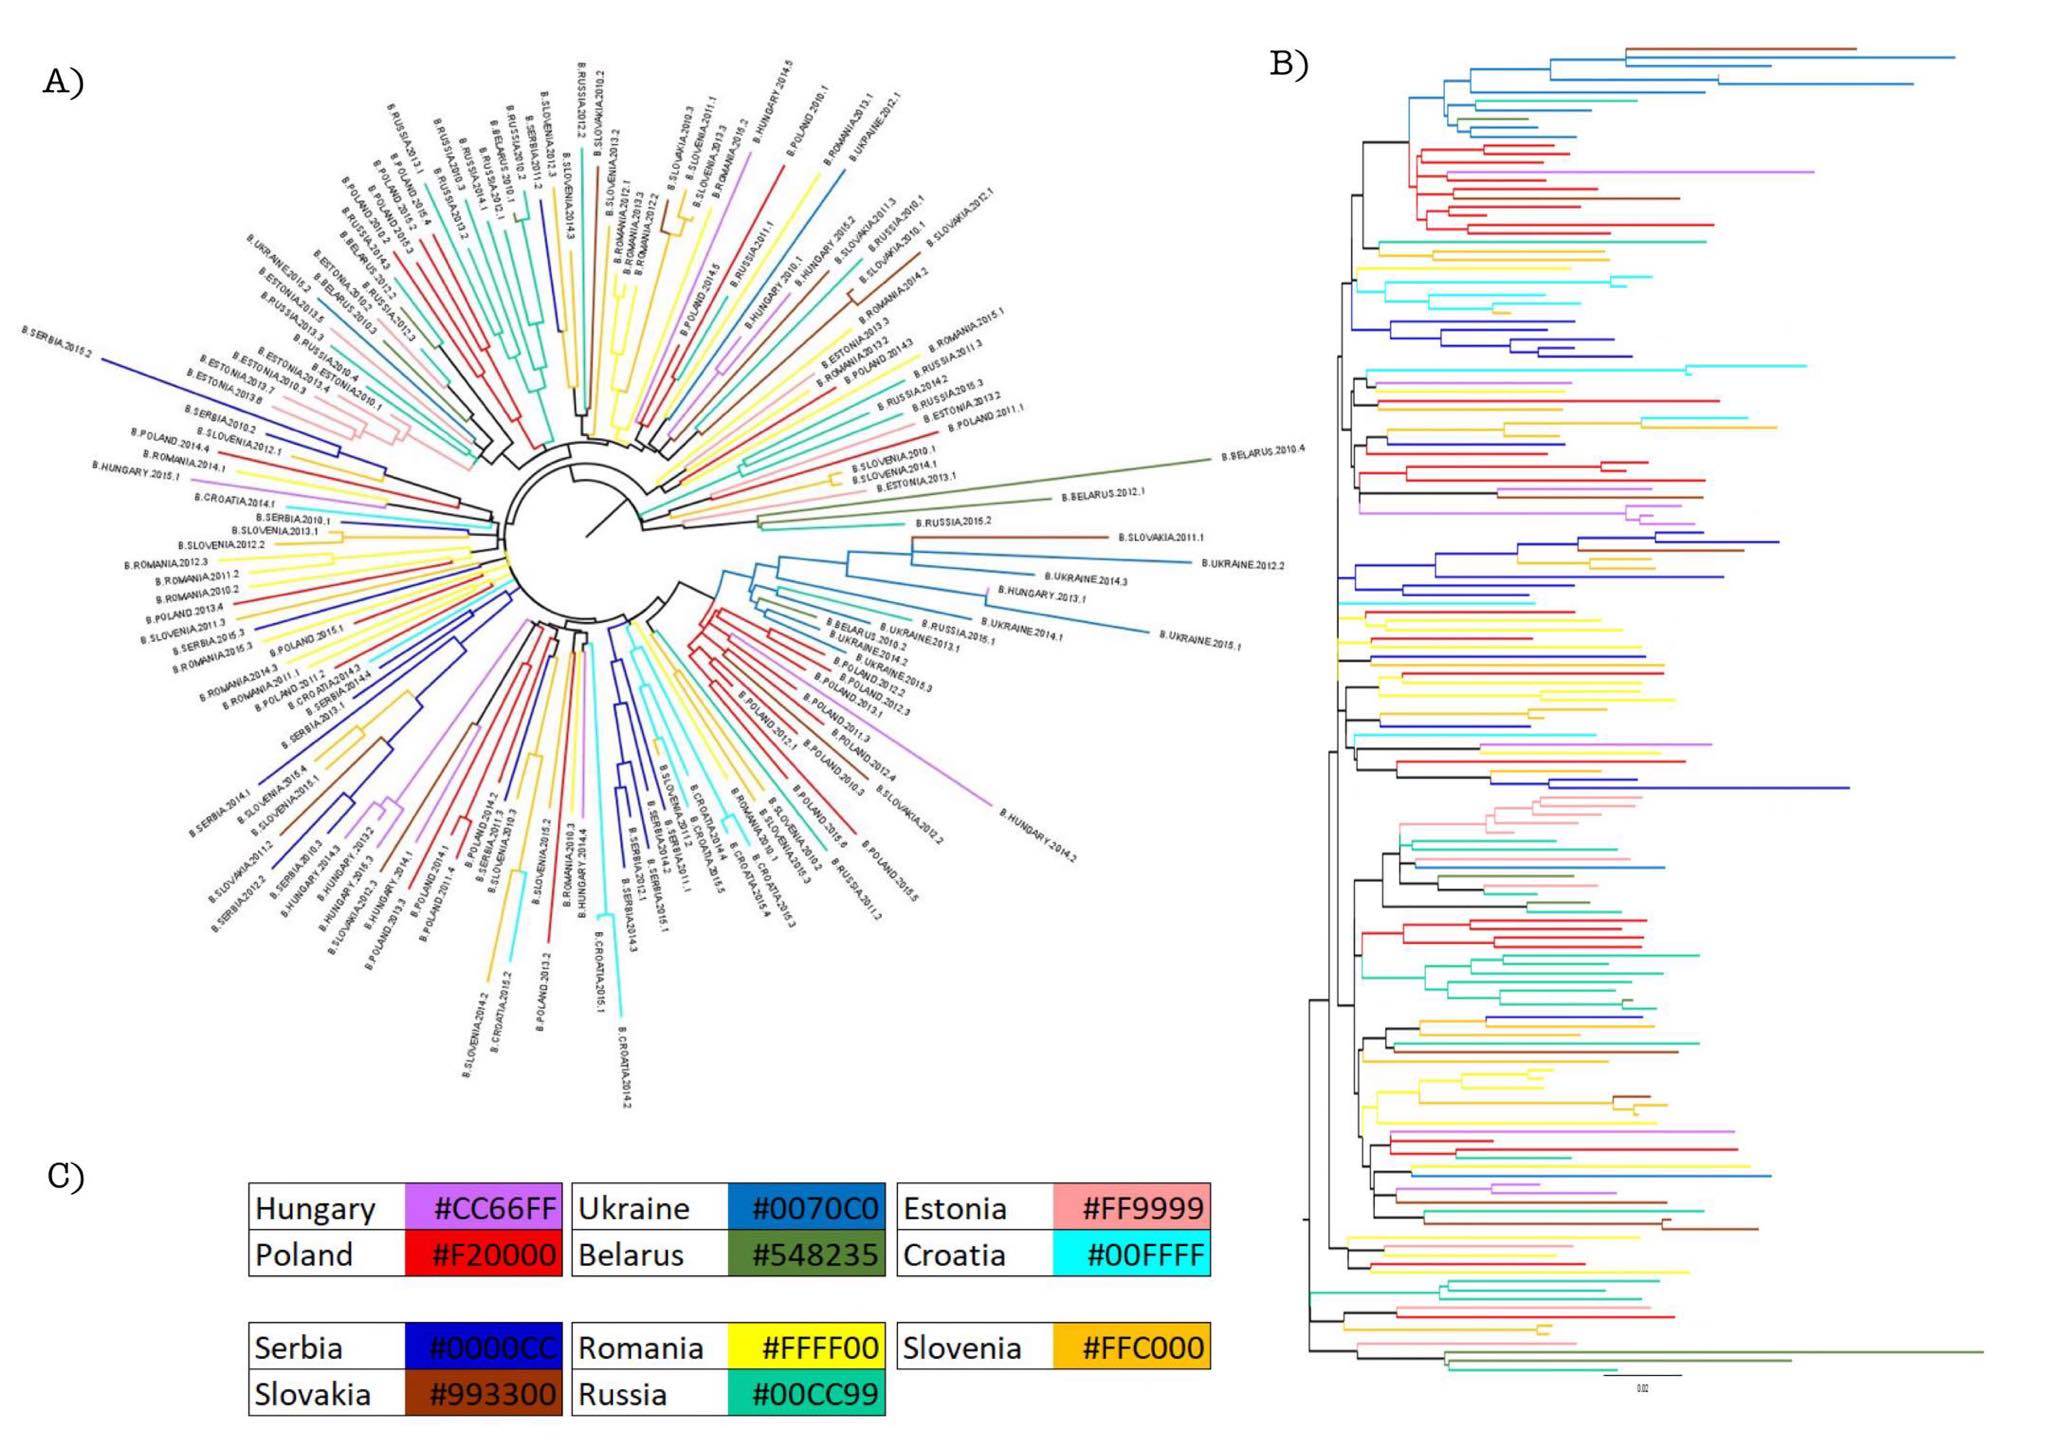
\includegraphics[width=0.8\textwidth]{images/after bootstrapping all.jpeg}
  \caption{Phylogenetic tree (after bootstrapping) aligned using MUSCLE in MEGA 11 and colored in the FigTree program. A) Polar tree layout which includes the names of the countries at the tip of the branches. B) Rectangular tree layout which does not include the name of the countries at the tip of the branches. C) Legend describing which color was used for which country.}
  \label{fig: No bootstrapping trees.}
\end{figure}

\section{Bootstrapping values}
Following the analysis in MEGA11, bootstrap values were calculated by the program, and a tree was produced. 
As the tree was built from 151 sequences, it was too large to fit on one page. 
To make it convenient, the tree  was split into 7 sections.
Figure 4.3 contains the first part of seven parts. 
A full phylogenetic tree that was obtained during the analysis was attached in the appendix (see. Figure A.1 and A.2)
\clearpage
Bootstrap values for the Serbian-Croatian-Slovenian clade were mostly over 90. 
The clade consists of four Croatian sequences, five Serbian sequences, one Slovenian sequence, and one sequence from Romania. 
Another high bootstrap value, which was 75, was found between two Polish sequences (B.POLAND.2012.2 and B.POLAND.2012.3) 
The rest of the bootstrap values within Figure 4.3 were below 70.

\begin{figure}[h]
  \centering
  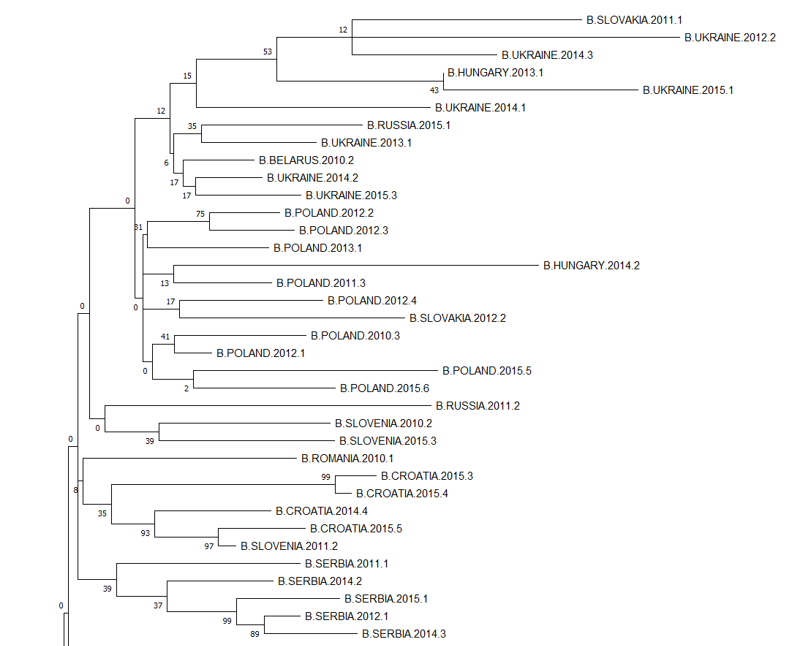
\includegraphics[width=0.7
\textwidth]{images/1.png}
  \caption{First part of the tree.}
  \label{fig: First part of the tree.}
\end{figure}
  
\begin{figure}[h]
  \centering
  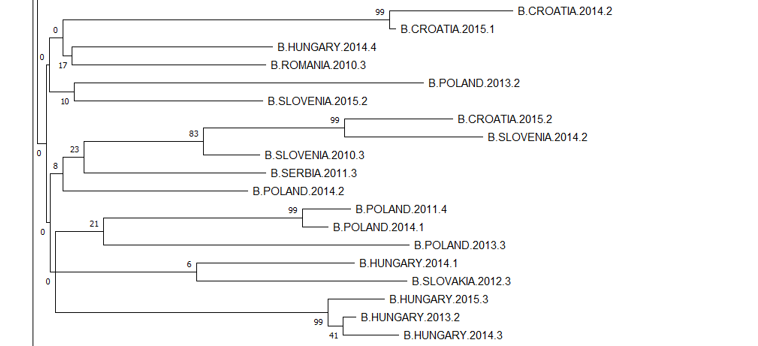
\includegraphics[width=0.7
\textwidth]{images/2.png}
  \caption{Second part of the tree.}
  \label{fig: Second part of the tree.}
\end{figure}

Figure 4.4 contains the second part of the tree.
High bootstrap values could be noticed between two Croatian sequences - B.CROATIA.2014.2 and B.CROATIA.2015.1 and were equal to 99.
The same value was seen between sequences B.CROATIA.2015.2 and B.SLOVENIA.2014.2. 
This branch was also connected to the Slovenian branch B.SLOVENIA.202010.3 with a bootstrap value equal to 83.
The bootstrap value between two Polish sequences – B.POLAND.2011.4 and B.POLAND.2014.1 also resulted in a high value equal to 99. 
A small Hungarian branch at the bottom of Figure 4.4 showed the bootstrap value of 99 between sequence B.HUNGARY.2015.3 and a branch containing sequences B.HUNGARY.2013.2 and B.HUNGARY.2014.3
The rest of the values did not exceed 70.

\begin{figure}[h]
  \centering
  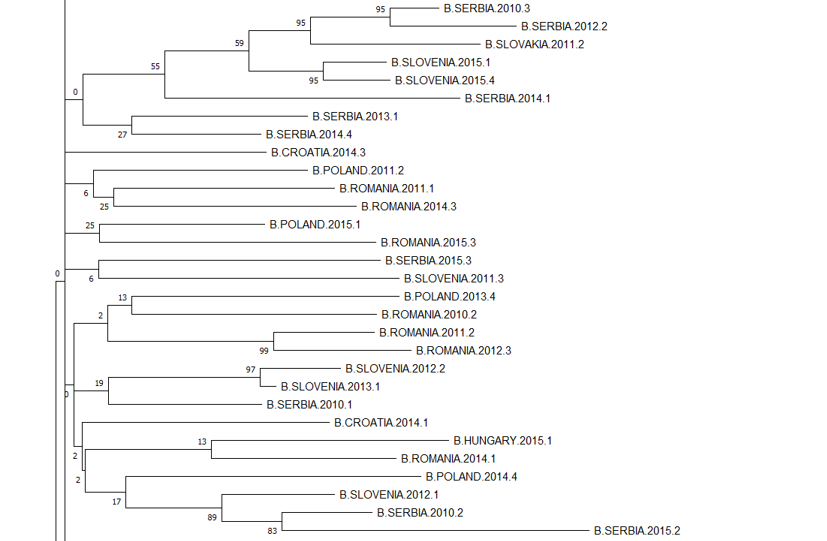
\includegraphics[width=0.7
\textwidth]{images/3.png}
  \caption{Third part of the tree.}
  \label{fig: Third part of the tree.}
\end{figure}

Figure 4.5 shows the third part of the tree. 
High bootstrap values could be found within the Serbian-Slovenian-Slovakian branch, which is located towards the top of the figure. 
A value of 95 was obtained between two Slovenian sequences, and between Serbian and Slovakian sequences. 
However, the bootstrap value between those branches was below 70.
A value of 99 was obtained between two Romanian sequences – B.ROMANIA.2011.2 and B.ROMANIA.2012.3.
A value of 97 was obtained between Slovenian sequences – B.SLOVENIA.2012.2 and B.SLOVENIA.2013.1.
Values over 80 were also obtained within the Serbian-Slovenian branch at the bottom of Figure 4.5.

\begin{figure}[h]
  \centering
  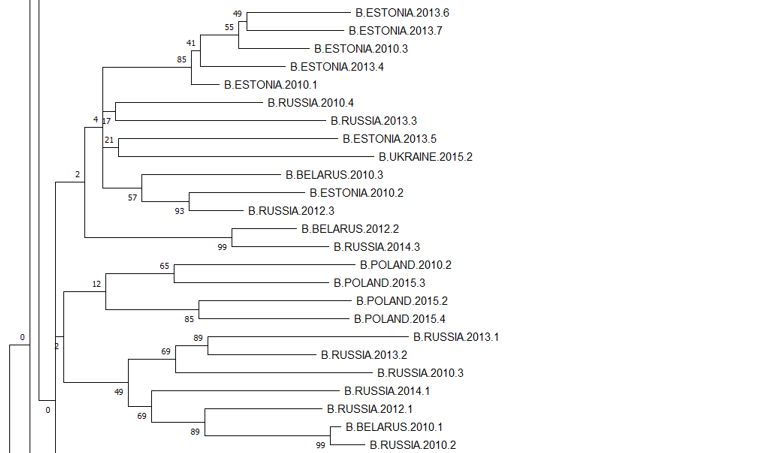
\includegraphics[width=0.7
\textwidth]{images/4.png}
  \caption{Fourth part of the tree.}
  \label{fig: Fourth part of the tree.}
\end{figure}

Figure 4.6 shows the fourth part of the tree. 
High bootstrap values could be found between Estonian sequence B.ESTONIA.2010.2 and Russian sequence B.RUSSIA.2012.3.
A value of 99 between Belarusian sequence B.BELARUS.2012.2 and Russian sequence B.RUSSIA.2014.3
A value of 85 was obtained between two Polish sequences – B.POLAND.2015.2 and B.POLAND.2015.4. 
Russian-Belarusian clade towards the bottom of Figure 4.6 also showed high bootstrap values as well, where the relativeness between Belarusian sequence B.BELARUS.2010.1 and B.RUSSIA.2010.2 gave a bootstrap value of 99. 

\begin{figure}[h]
  \centering
  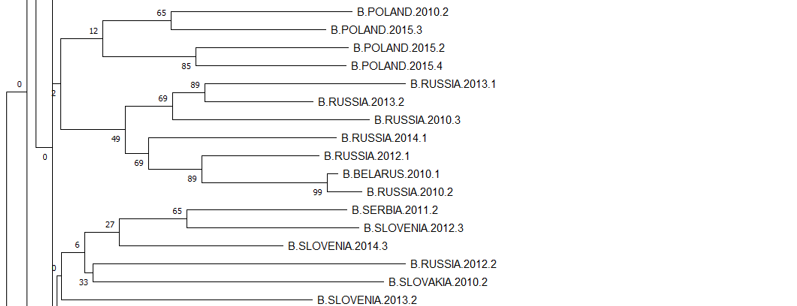
\includegraphics[width=0.7
\textwidth]{images/5.png}
  \caption{Fifth part of the tree.}
  \label{fig: Fifth part of the tree.}
\end{figure}

Figure 4.7 shows the fifth part of the tree.
High bootstrap values were noted between two Polish sequences - B.POLAND.2015.2 and B.POLAND.2015.4 and were equal to 85.
A value of 89 was obtained between two Russian sequences - B.RUSSIA.2013.1 and B.RUSSIA.2013.2.
A value of 89 was also obtained between Russian sequence B.RUSSIA.2012.1 and the Russian-Belarusian branch containing sequences B.BELARUS.2010.1 and B.RUSSIA.2010.2. 
The bootstrap value between those two sequences was also high and was equal to 99. 
\vspace{0.5in}
\begin{figure}[h]
  \centering
  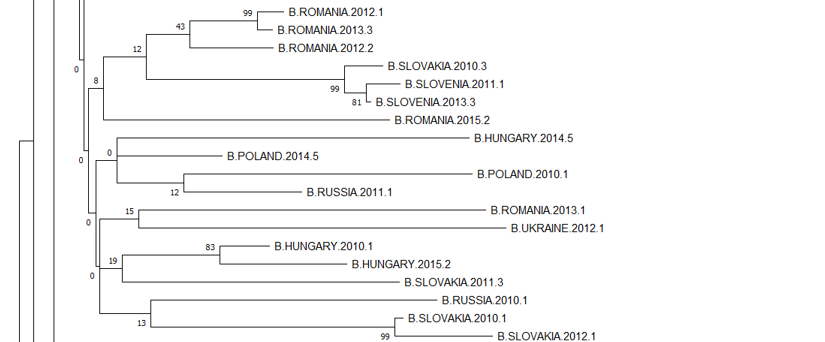
\includegraphics[width=0.7
\textwidth]{images/6.png}
  \caption{Sixth part of the tree.}
  \label{fig: Sixth part of the tree.}
\end{figure}

Figure 4.8 shows the sixth part of the tree.
High bootstrap values were noticed between two Romanian sequences – B.ROMANIA.2012.1 and B.ROMANIA.2013.3 and were equal to 99.
A small Slovenian – Slovakian clade containing Slovakian sequence B.SLOVAKIA.2010.3 and a branch containing sequences B.SLOVENIA.2011.1 and B.SLOVENIA.2013.3 had a bootstrap value of 99 and the value of 81 was obtained within the Slovenian branch. 
A value of 83 was obtained between two Hungarian sequences – B.HUNGARY.2010.1 and B.HUNGARY.2015.2.
Towards the bottom of Figure 4.8, there was a Slovakian branch containing sequences B.SLOVAKIA.2010.1 and B.SLOVAKIA.2012.1 which gave the result of 99.

\begin{figure}[h]
  \centering
  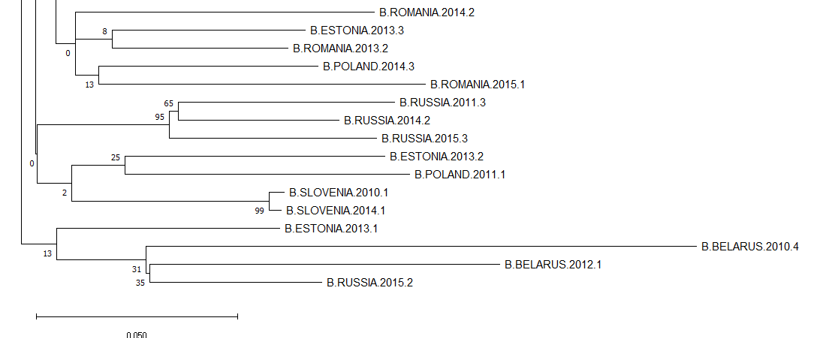
\includegraphics[width=0.7
\textwidth]{images/7.png}
  \caption{Seventh part of the tree.}
  \label{fig: Seventh part of the tree.}
\end{figure}

Figure 4.9 shows the last, seventh part of the tree.
The only high bootstrap value was obtained between the Russian sequence B.RUSSIA.2014.2 and the Russian branch containing sequences B.RUSSIA.2015.1 and B.RUSSIA.2014.2, however, the value between sequences within this branch was below 70. 
The rest of the bootstrap values did not exceed 70.




